% Unofficial ERC Starting Grant LaTeX template 
% Source: http://www.arj.no/2013/02/03/erc-stg-latex/
%
\documentclass[oneside, a4paper, onecolumn, 11pt]{article}
%up to 15 pages without budget table and references
%%% PACKAGES %%%

\usepackage[left=2cm,top=2cm,bottom=1.5cm,right=2cm]{geometry}
\usepackage{hyperref}
\usepackage[utf8]{inputenc}
\usepackage{graphicx} 		% Add graphics capabilities
\usepackage{amsmath}  		% Better maths support
\usepackage{natbib}	% bibliography style
\setlength{\bibsep}{0.0pt}
\usepackage{eurosym}
\usepackage{comment}
\usepackage{floatrow}
\usepackage{afterpage}
\usepackage{color,xcolor}
\definecolor{absolutezero}{rgb}{0.0,0.28,0.73}
\definecolor{bluetiful}{rgb}{0.24,0.41,0.91}
\definecolor{aoenglish}{rgb}{0.0,0.5,0.0}
\definecolor{imperialred}{rgb}{0.93,0.16,0.22}
\usepackage{multirow}
\usepackage{colortbl}
\usepackage{lmodern,textcomp}
\usepackage{relsize} % e.g. used for \mathsmaller
\usepackage{caption}
\usepackage{array}
\usepackage{tikz}
\usetikzlibrary{fit,shapes, arrows}
\usepackage{chemfig}
\usetikzlibrary{decorations.markings}


\linespread{1.0}

% To fix list things: 
\usepackage{enumitem}
\setitemize{noitemsep,topsep=0pt,parsep=0pt,partopsep=0pt,leftmargin=*}
\usepackage{amssymb}
\renewcommand{\labelitemi}{\tiny$\blacksquare$}

\usepackage{nopageno}
\usepackage{enumitem}

\usepackage{fancyhdr}
\pagestyle{fancy}
\renewcommand{\headrulewidth}{0pt} % Remove line at top

\usepackage{todonotes}
\usepackage{subcaption}

 
\lhead{}
\rhead{}
\chead{\textbf{Exploring alternative formulations of Smoothed Particle Hydrodynamics for complex fluids and solids}}
\cfoot{\thepage}

\newenvironment{itemize*}%
  {\begin{itemize}%
    \setlength{\itemsep}{0pt}%
    \setlength{\parskip}{0pt}}%
  {\end{itemize}}

\renewcommand\thesection{\alph{section}}
%\renewcommand\thesubsection{\thesection.\arabic{subsection}}
\renewcommand\thesubsection{\thesection.\arabic{subsection}}
%\def\thesection{\arabic{subsection}}



\usepackage{enumitem}

%\renewcommand{\thesubsection}{\thesection.\alph{subsection}}
%\renewcommand{\thesubsection}{\Alph{subsection}}
\newcommand{\EE}{\mathbf{E}}
\newcommand{\DD}{\mathbf{D}}
\newcommand{\BB}{\mathbf{B}}
\newcommand{\HH}{\mathbf{H}}
\renewcommand{\AA}{\mathbf{A}}
\newcommand{\PP}{\mathbf{P}}
\newcommand{\ppi}{\boldsymbol{\pi}}
\newcommand{\oomega}{\boldsymbol{\omega}}
\newcommand{\MM}{\mathbf{M}}
\newcommand{\JJ}{\mathbf{J}}
\newcommand{\ii}{\mathbf{i}}
\newcommand{\vv}{\mathbf{v}}
\newcommand{\mm}{\mathbf{m}}
\newcommand{\xx}{\mathbf{x}}
\newcommand{\XX}{\mathbf{X}}
\newcommand{\yy}{\mathbf{y}}
\newcommand{\WW}{\mathbf{W}}
\newcommand{\diff}{\mathrm{d}}
\newcommand{\A}[2]{A^{\mathsmaller#1}_{\ \, #2}}
\newcommand{\nn}{\mathbf{n}}
\newcommand{\II}{\mathbf{I}}
\newcommand{\FF}{\mathbf{F}}
\newcommand{\QQ}{\mathbf{Q}}
\newcommand{\CC}{\mathbf{C}}
\renewcommand{\SS}{\mathbf{S}}
\newcommand{\eeta}{\boldsymbol{\eta}}
\renewcommand{\aa}{\mathbf{a}}
\newcommand{\qq}{\mathbf{q}}
\newcommand{\BBB}{\boldsymbol{\mathcal{B}}}
\newcommand{\dWW}{\mathrm{d}\mathbf{W}}
\newcommand{\OO}{\mathbf{1}}
\newcommand{\TT}{\mathbf{2}}
\newcommand{\intd}{\int\,\diff}
\newcommand{\rr}{\mathbf{r}}
\newcommand{\pp}{\mathbf{p}}
\newcommand{\LL}{\mathbf{L}}
\newcommand{\ee}{\mathbf{e}}

\renewcommand{\ss}{\mathbf{s}}

%%% COMMANDS %%%

\begin{document}
%%% Content

%\begin{center}
%\large{\textbf{
%ERC Starting Grant 2021\\
%Part B2}}
%\end{center}


%\begin{figure}[ht]
%    \centering
%    \includegraphics[scale=0.6]{corpse.jpg}
%    \caption{A galvanised corpse \citep{corpse}. As the usual parabolic equations for electrochemistry are purely dissipative, they inevitably monotonously approach their terminal state, thermodynamic equilibrium. On the other hand, hyperbolic electrochemistry (Inertial Electrochemistry) would be equipped with inertial effects allowing the systems to evolve no only irreversibly towards the equilibrium, but also reversibly.}
%\end{figure}
%\afterpage{\clearpage}

%\tableofcontents


%\end{enumerate}
\begin{center}
    \vspace*{\fill}
    {\Huge\bfseries Application}
    \vspace*{\fill}
\end{center}
%\clearpage

I am applying for the Student Faculty Grant "Exploring alternative formulations of Smoothed Particle Hydrodynamics for complex fluids and solids" under the Mathematical Institute of Charles University.
\vspace{\fill}
\begin{itemize}

\item \textbf{Applicant}: Michael Monček, $3^{\text{rd}}$ year Bachelor student of Mathematical Modelling, intending to continue with a Master’s degree in Mathematical Modelling in Physics and Technology at the Mathematical Institute of Charles University.



\begin{figure}[H]
    \centering
    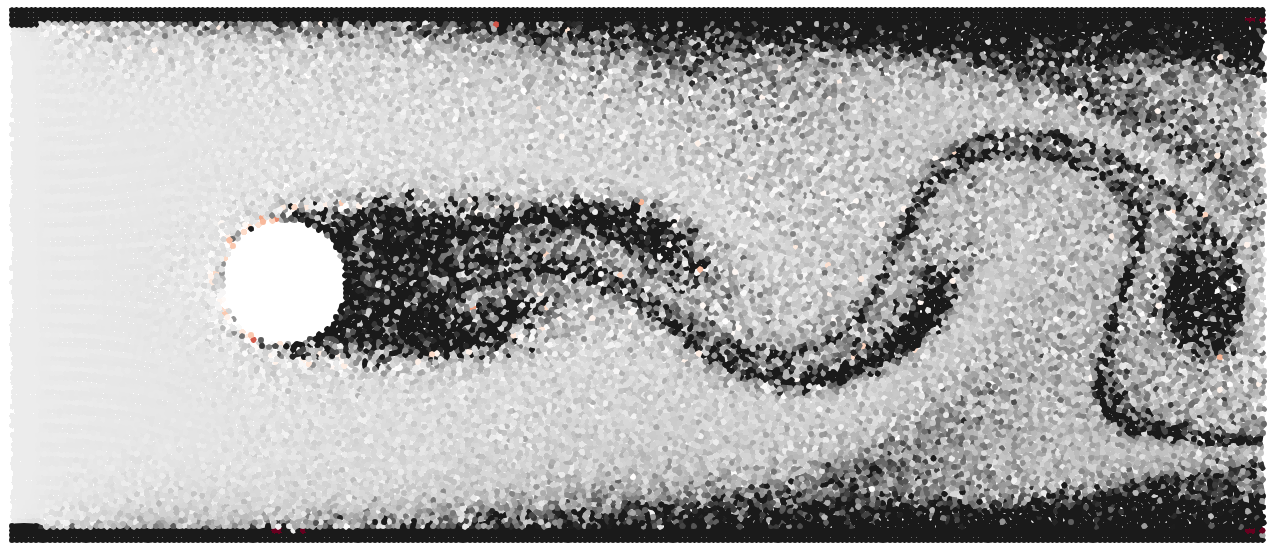
\includegraphics[width=0.85\linewidth]{distortion_grey_highres.png}
    \caption{The distortion field in the flow around cylinder benchmark simulated using SHTC-SPH.}
    \label{fig:enter-label}
\end{figure}

\item \textbf{Introduction}: Complex fluids and solids can be described by the Symmetric Hyperbolic Thermodynamically Compatible (SHTC) equations. These equations have a Hamiltonian structure and are advantageous in problems with large deformations and shock waves. One of the state variables in the SHTC equations is the distortion field (close to the inverse of the deformation gradient). Recently, a new numerical method solving the SHTC equations was developed based on the Smoothed Particle hydrodynamics (SPH) \cite{kincl-unified}. 

However, in a later work \cite{hutter-pavelka}, an alternative definition of the discrete distortion that is useful when adding noise to the SHTC equations (to be applied in continuum physics of nanomaterials) was developed. In this definition, the discrete distortion is defined as the minimizer of the following functional, 
\begin{equation*}
	D = \sum_\alpha\sum_\beta w_\alpha w_\beta ||\mathbf{R}_{\alpha\beta} - \mathbf{A} \cdot \mathbf{r}_{\alpha\beta}||^2,
\end{equation*}
where $\mathbf{R}_{\alpha\beta}$ is the difference between the Lagrangian positions of the particles $\alpha$ and $\beta$, $\mathbf{r}_{\alpha\beta}$ is the difference between Eulerian positions, and $w_\alpha(\mathbf{r})$ is a weight kernel of particle $\alpha$ (for instance the SPH kernel). The minimization of this functional leads to a discrete distortion field $\mathbf{A}$ that may be more suitable for SPH simulations of SHTC equations. 

If the numerical SPH-based method becomes compatible with the new definition, it would be possible to simulate nanomembranes and other nanomaterials, where fluctuations play an important role, by the method. 

	\item \textbf{Goal}: 
	\begin{itemize}
	\item Reformulation of the numerical framework from \cite{kincl-unified} to the new definition of the distortion field.
	\item Comparison of the two formulations of the SHTC equations in SPH simulations.
	\end{itemize}


\item \textbf{Specific tasks and Work Plan}: 
\begin{enumerate}
\item \textbf{July – December 2025}: %Use the definition of distortion from \cite{hutter-pavelka} to reformulate the SPH method from \cite{kincl-unified}.
Reformulation of the SPH method to incorporate the new definition of distortion
\item \textbf{July – December 2025}: As the formulation of the discrete dynamics in \cite{kincl-unified} is simplified, an attempt to use the full system of equations without neglecting the denominator of the discrete distortion matrix.

\item \textbf{January – April 2026}: Comparative simulations of benchmark problems simulated in \cite{kincl-unified}, for instance the Beryllium plate benchmark or lid-driven cavity. 
\item \textbf{April – May 2026}: If the tests are successful, extension to fluid-structure interaction problems
(e.g. Turek-Hron bechmark \cite{turek-hron}).

\item \textbf{May – July 2026}: Final analysis, documentation, and preparation of research output.
\end{enumerate}

\item \textbf{Project Duration}:
\begin{itemize*}
\item \textbf{Start Date}: July 1, 2025
\item \textbf{End Date}: July 1, 2026
\end{itemize*}

\item \textbf{Relation to Bachelor’s Thesis}:
The topic of this project is related to the applicant's Bachelor thesis, which concerns numerical simulation of
fluid-structure interaction problems using the numerical method developed in \cite{kincl-unified}.
The SFG project is designed to go beyond the scope of the thesis by exploring new formulations and applications.
This project also serves as a foundation for future research in the applicant’s planned Master’s studies at the Mathematical Institute of Charles University.


\item \textbf{Supervisor}: Michal Pavelka (Mathematical Institute of Charles University), pavelka@karlin.mff.cuni.cz

\end{itemize}





%%% Bibliography
\bibliographystyle{abbrv}  % ama, nar, alpha, plain, chicago, abbrv, siam
\bibliography{library.bib}


\vspace{2cm}

\begin{tabular*}{\textwidth}{@{\extracolsep{\fill}} l r}
Prague, May 14, 2025 & 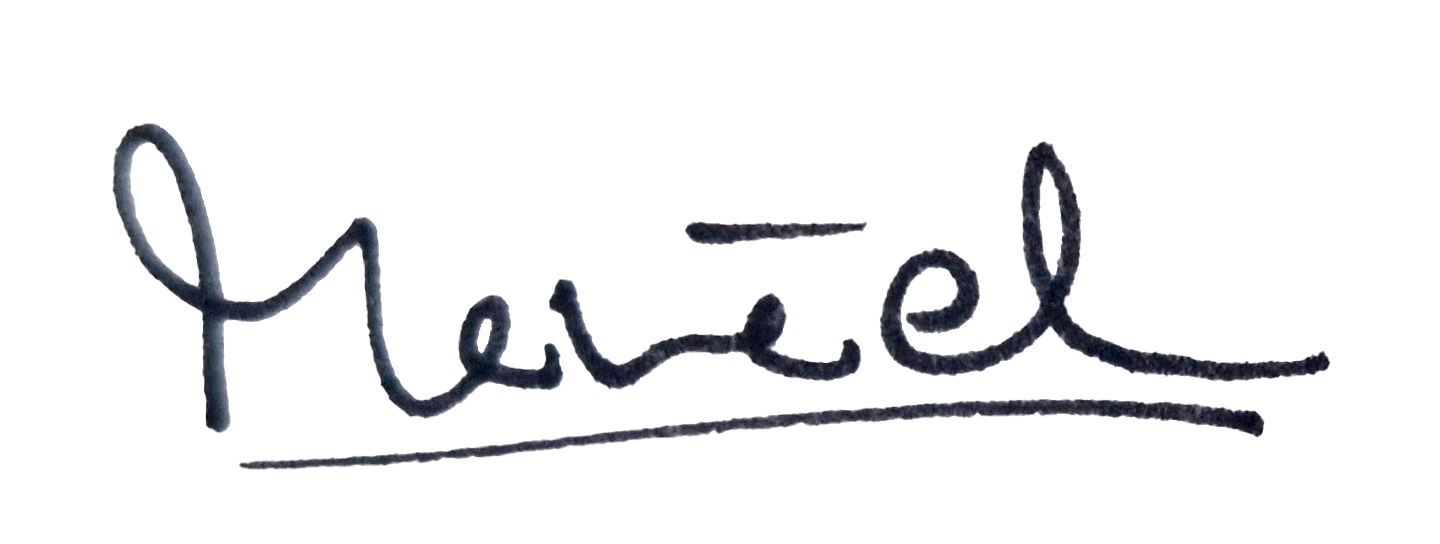
\includegraphics[height=1.5cm]{signature.png} \\
& Michael Monček
\end{tabular*}

\newpage

In our alternative formulation, the distortion field $\AA$ at point $\xx$ is defined as a minimizer of the following functional:
\begin{equation}
    D_{\xx}(\AA) = \sum_a \sum_b w_a(\xx) w_b(\xx) \| \XX_{ab} - \AA \xx_{ab} \|^2
\end{equation}
where $w_a(\xx) = w(\xx - \xx_a)$ and $\|\vv\|^2 = \vv \cdot \vv$ is the standard vector product.\\

Evaluating the sufficient condition for the minimum of $D_{\xx}(\AA)$ yields:
\begin{equation}
    \frac{\diff D_{\xx}(\AA)}{\diff \AA} = \frac{\diff}{\diff\AA} \sum_a \sum_b w_a(\xx) w_b(\xx) \left( \XX_{ab} - \AA \xx_{ab} \right)^T \left( \XX_{ab} - \AA \xx_{ab} \right) =
    \sum_a \sum_b w_a(\xx) w_b(\xx) \frac{\diff}{\diff \AA} \left(
    \right)
\end{equation}
\begin{subsection} {Time evolution of the distortion field}
The distortion field at point $a$ can be explicitely written as \begin{equation}
    \AA_a = \PP_a \QQ_a^{-1}
\end{equation}
where \begin{equation}
    \PP_a = \left( \sum_b w_{ab} \XX_{ab} \otimes \xx_{ab} \right) \text{ and }
    \QQ_a =  \left( \sum_b w_{ab} \xx_{ab} \otimes \xx_{ab} \right)
\end{equation}
The differential of the distortion field is then \begin{equation}
    \diff \AA = \diff \PP \QQ^{-1} + \PP \diff \QQ^{-1} =
    \diff \PP \QQ^{-1} - \PP \QQ^{-1} \diff \QQ \QQ^{-1} 
\end{equation}

If we use the approximations \begin{equation}
    \dot{\xx}_a \approx \dot{\xx}_b + \nabla \vv \Big|_a \cdot \xx_{ab} \text{ and } 
    \XX_{ab} \approx \AA_a \xx_{ab}
\end{equation} 
this expression simplifies to: 
\begin{equation}
    \diff \AA_a = - \AA_a \LL_a = - \AA_a \nabla \vv \Big|_a
\end{equation}
which is the evolution equation for the distortion field in the SHTC equations.\\
On the other hand if we do not choose to approximate $\dot{\xx}_a$ we get the following evolution equation: 
\begin{equation}
    \diff \AA_a = - \AA_a \left( \sum_b w_{ab} \diff \xx_{ab} \otimes \xx_{ab}\right)
    \left( \sum_b w_{ab} \xx_{ab} \otimes \xx_{ab}\right)^{-1}
\end{equation}
We can than define the SPH velocity gradient at point $a$ as: 
\begin{equation}
    \LL_a := \left( \sum_b w_{ab} \vv_{ab} \otimes \xx_{ab}\right)
    \left( \sum_b w_{ab} \xx_{ab} \otimes \xx_{ab}\right)^{-1}
\end{equation}

\todo[inline]{Do we know if this definition of velocity gradient approximates the real velocity gradient well?}

If we choose not to approximate at all we get the following expression:
\begin{equation}
    \begin{aligned}
    \diff \AA_a = - \AA_a \LL_a +
    \left(\sum_b \nabla w_{ab} \cdot \diff \xx_{ab} \left(\XX_{ab} - \AA_a \xx_{ab}
    \right) \otimes \xx_{ab}\right)\QQ_a^{-1} +\\
    \left(\sum_b w_{ab} \left(\XX_{ab} - \AA_a \xx_{ab}
    \right) \otimes \diff \xx_{ab}\right)\QQ_a^{-1}
    \end{aligned}
\end{equation}

\end{subsection}
\begin{subsection} {Equations of motion}
Let $U_h = \sum_b \epsilon_b$ be the discrete total energy of the system, $\epsilon_b$ is the specific energy 
density of particle $b$. We assuem that the specific energy density depends on the density $\rho$ and the 
distortion field $\AA$. The total differential of the total energy is then: 
\begin{equation}
    \begin{aligned} 
    \diff U_h = \sum_a m_a \epsilon_{\AA_a} : \diff \AA_a + \sum_a m_a \epsilon_{\rho_a} \diff \rho_a
    = \sum_a m_a \epsilon_{\rho_a} \left( \sum_b m_b \diff \xx_{ab} \cdot \nabla w_{ab} \right)
    + \sum_a m_a \epsilon_{\AA_a} : \left( - \diff \AA_a \right) \\
    = \sum_{a,b} m_a m_b  \left( \epsilon_{\rho_a} \nabla w_{ab} \cdot \diff 
    \xx_{ab} - \frac{1}{m_b} \epsilon_{\AA_a} : \AA_a 
    \left( w_{ab} \diff \xx_{ab} \otimes \xx_{ab}\right) \QQ_a^{-1}
    \right) \\
    = -\sum_{a,b} m_a m_b \left(\frac{1}{m_b} w_{ab} \Pi_a \xx_{ab} - 
    \epsilon_{\rho_a} \nabla w_{ab}  \right) \cdot \diff \xx_{ab}\\
    = -\sum_{a,b} m_a m_b \left(\frac{1}{m_b} w_{ab} \Pi_a \xx_{ab} - 
    \epsilon_{\rho_a} \nabla w_{ab}  \right) \cdot \left(\diff \xx_a - \diff \xx_b\right)\\
    = -\sum_{a,b} m_a m_b \left(\frac{1}{m_b} w_{ab} \Pi_a \xx_{ab} - 
    \epsilon_{\rho_a} \nabla w_{ab}  \right) \cdot \diff \xx_a \\
    - \sum_{b,a} m_b m_a \left(\frac{1}{m_a} w_{ba} \Pi_b \xx_{ab} - 
    \epsilon_{\rho_b} \nabla w_{ab}  \right) \cdot \diff \xx_a\\ 
    = -\sum_{a,b} m_a m_b \left[ w_{ab} \left( \frac{\Pi_a}{m_b} + \frac{\Pi_b}{m_a} \right) \xx_{ab} 
    - \left( \epsilon_{\rho_a} + \epsilon_{\rho_b} \right) 
    \nabla w_{ab} \right] \cdot \diff \xx_a
    \end{aligned}
\end{equation} where $\Pi_a = \AA_a^T \epsilon_{\AA_a} \QQ_a^{-T}$.\\ 
Using Newton's second law $m \dot{\xx} = - \frac{\diff U}{\diff \xx}$ we get the following equations of motion: 
\begin{equation} 
    m_a \dot{\vv}_a = \sum_b m_a m_b \left[ w_{ab} \left( \frac{\Pi_a}{m_b} + \frac{\Pi_b}{m_a}\right) 
    \xx_{ab} - \left( \epsilon_{\rho_a} +
    \epsilon_{\rho_b} \right) \nabla w_{ab} \right] 
\end{equation} 
%{
\todo[inline]{These equations are different from the equations Ondra originally proposed
 and from those in the example code rod.jl something is wrong here.} 

Let us assume that the inner energy $\epsilon$ decomposes into bulk and shear part as $\epsilon(\rho, \AA) = 
\epsilon_0(\rho) + \epsilon_s(\AA)$. 
We will use the following quadratic relation for the bulk component:
\begin{equation}
    \begin{aligned}
    \epsilon_0(\rho) = c_0^2 / 2 \left(\frac{\rho_0}{\rho} - 1\right)^2\\
    \epsilon_0'(\rho) = c_0^2 \left(\frac{\rho_0}{\rho} - 1\right)
    \left(- \rho_0 / \rho^2 \right) = c_0^2 \rho_0 \left( \frac{1}{\rho^2}
    - \frac{\rho_0}{\rho^3}\right)
    \end{aligned}
\end{equation}
For the shear component we will use the following equation:
\begin{equation}
    \begin{aligned}
    \epsilon_s(\AA) = \frac{c_s^2}{4}\| \text{dev}(\AA^T\AA) \|^2_F\\
    \epsilon_s'(\AA) = c_s^2 \AA \text{dev}(\AA^T\AA)
    \end{aligned}
\end{equation}
We can than write the $\Pi_a$ as:
\begin{equation}
    \Pi_a = c_s^2 \AA^T_a \AA_a \text{dev}(\AA_a^T \AA_a) \QQ_a^{-T} 
\end{equation}

We can treat the density $\rho$ in two ways. The first one is the standard SPH density approximation:
\begin{equation}
    \rho_a = \sum_b m_b w_{ab}
\end{equation}
The second way is the following relation:
\begin{equation}
    \rho_a = \rho_0 \det(\AA_a)
\end{equation}

With this we have derived the following system of equations for the 
Particle distortion SPH-SHTC:

\begin{subequations}
    \begin{equation}
        \dot{\xx}_a = \vv_a\\
    \end{equation}
    \begin{equation}
        \dot{\vv}_a = \sum_b m_b \left[ w_{ab} \left( \frac{\Pi_a}{m_b} + 
        \frac{\Pi_b}{m_a}\right) \xx_{ab} - \left( \epsilon_{\rho_a} +
        \epsilon_{\rho_b} \right) \nabla w_{ab} \right]\\
    \end{equation}
    \begin{equation} 
        \AA_a = \left( \sum_b w_{ab} \XX_{ab} \otimes \xx_{ab} \right) 
        \left( \sum_b w_{ab} \xx_{ab} \otimes \xx_{ab} \right)^{-1}
    \end{equation}
\end{subequations}

THe only thing to see now is whether is works or not xD 
We have neglected some terms so here they are (using the notation $
\ee_{ab} = \XX_{ab} - \AA_a \xx_{ab}$):

\begin{equation}
    \sum_a m_a \epsilon_{\AA_a} :
    \left(\sum_b w_{ab} \ee_{ab} \otimes \diff \xx_{ab}\right)\QQ_a^{-1} =
    \sum_{a,b} w_{ab} \left(m_a \Pi'_a \ee_{ab} - 
    m_b \Pi'_b \ee_{ba}\right) \cdot \diff \xx_a
\end{equation}

\begin{equation}
    \sum_a m_a \epsilon_{\AA_a} :
    \left(\sum_b \nabla w_{ab} \cdot \diff \xx_{ab} 
    \ee_{ab} \otimes \xx_{ab}\right)\QQ_a^{-1}
    = \sum_{a,b} \left( \left(m_a \Pi'_a \ee_{ab} - m_b \Pi'_b \ee_{ba}\right) 
    \cdot \xx_{ab}\right) \nabla w_{ab} \cdot \diff \xx_a
\end{equation}

where $\Pi'_a = c_s^2 \QQ_a^{-1} \text{dev}(\AA_a^T \AA_a) \AA_a^T$ also note that
$\Pi_a = (\Pi'_a \AA_a)^T$ furthemore we will write 
$\ss_{ab} = \left(m_a \Pi'_a \ee_{ab} - m_b \Pi'_b \ee_{ba}\right)$.

The full form of the evolution equation for velocity then reads:
\begin{equation}
    \dot{\vv}_a = \sum_b m_b \left[ w_{ab} \left( \frac{\Pi_a}{m_b} + 
    \frac{\Pi_b}{m_a}\right) \xx_{ab} - \left( \epsilon_{\rho_a} +
    \epsilon_{\rho_b} \right) \nabla w_{ab} \right]\
\end{equation}

\end{subsection} 

\begin{subsection} {Beryllium plate}
Remember the terms we neglected earlier because they were small? They were not that small after all, lets
take a look at what happens in the Beryllium plate benchmark withouth them.
\begin{figure}[H]
    \centering
    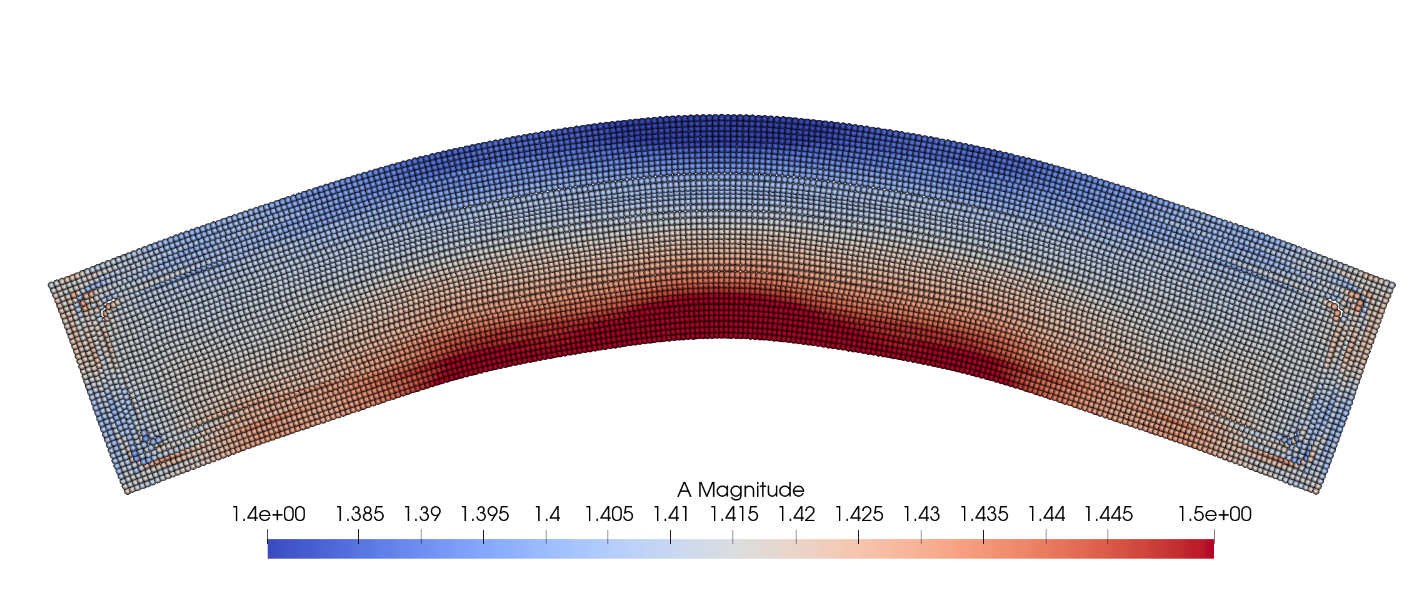
\includegraphics[width=0.85\linewidth]{plate1.png}
    \caption{For small deformations and large support radius it seems to 
    work at first.}
    \label{fig:plate1}
\end{figure}

\begin{figure}[H]
    \centering
    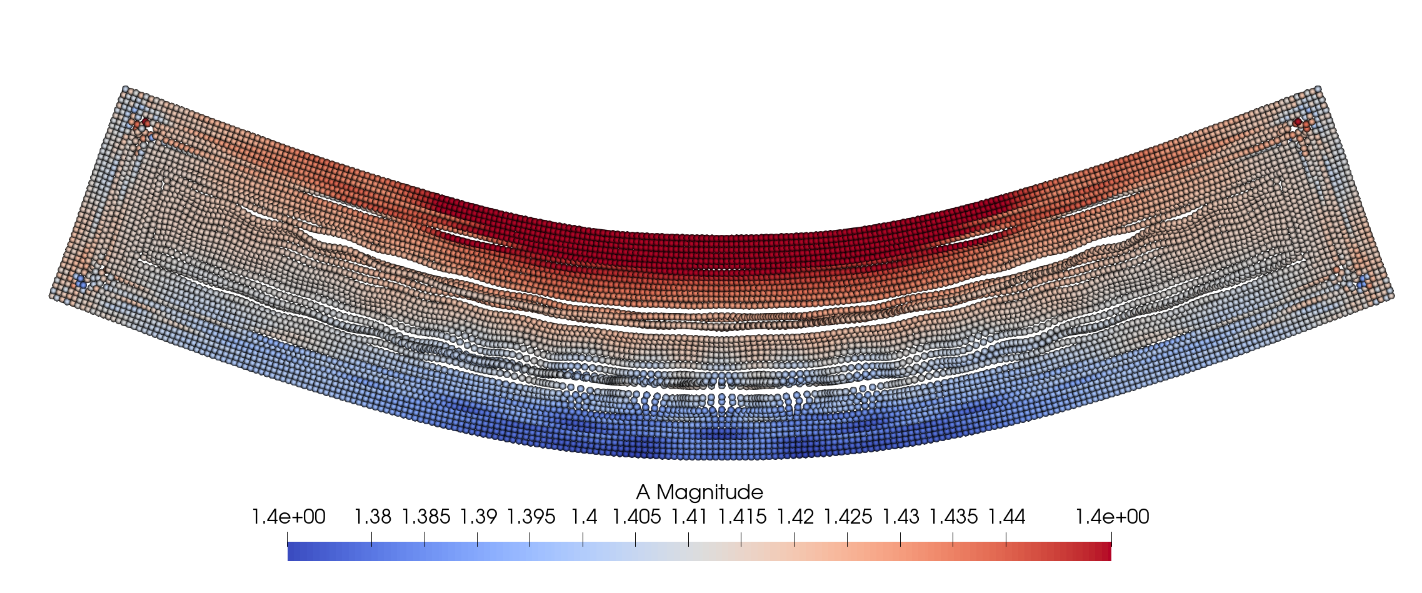
\includegraphics[width=0.85\linewidth]{plate2.png}
    \caption{However, even with support radius $h = 20dr$ (which is huge)
    the simulation becomes unstable after some time. 
    This does not seem to be tensile instability as the pressure is positive
    in the problematic places. It more has to do with this approximation 
    $\XX - \AA \xx \approx 0$.}
    \label{fig:plate2}
\end{figure}



\todo[inline]{TODO: Add the missing terms to the evolutoin equation for distorion to 
see what happens.}
\end{subsection}

\end{document}
